%=========================================================================
% fig-parallel-node-blocking.tex
%=========================================================================

\begin{figure}[h]

  \centering
  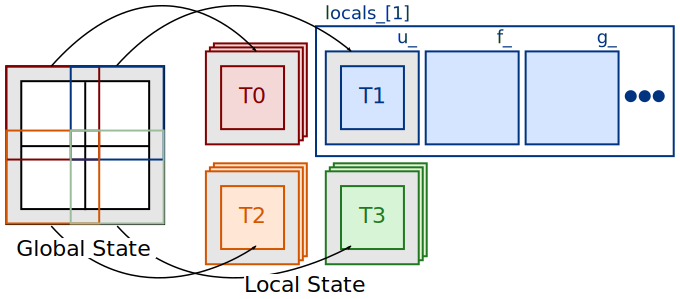
\includegraphics[width=0.9\tw]{fig-parallel-node-blocking.svg.pdf}

  \caption{\textbf{Parallelizing Computation Using Per-Thread Local State --}
    In this example, the global grid is divided into four local blocks,
    each of which is copied to per-thread memory allocated separately
    from the global grid. The LocalState class encapsulates all vectors
    in a local block including \texttt{u\_}, \texttt{f\_}, \texttt{g\_},
    \texttt{ux\_}, \texttt{uy\_}, \texttt{fx\_}, \texttt{gy\_}, and
    \texttt{v\_}. Each thread is only responsible for computing the
    solution of the live cells (i.e., non-gray area) in its local
    block. In order to do so, the vectors in the ghost cells (i.e., gray
    area) must be used. Note that the ghost cells of one local block
    overlap with the live cells of other local blocks grid, causing
    redundant computation. }

  \label{fig-parallel-node-blocking}

\end{figure}
